\documentclass[journal]{IEEEtran}
\usepackage{graphicx}
\usepackage{adjustbox}
\usepackage{amsmath,amssymb}
\usepackage{url}
\usepackage[T1]{fontenc}
\usepackage{textcomp}
\usepackage{microtype}
\usepackage{hyperref}
\hypersetup{hidelinks}
\graphicspath{{../}}
\sloppy
\begin{document}
\title{The Cost of Stale Telemetry in Traffic Engineering: Learned Policies, Re-Tuned Heuristics and ECMP}
\author{Dev~Nambiar,~\IEEEmembership{Vellore Institute of Technology, Vellore, India}%
\thanks{Manuscript not yet submitted. Corresponding e-mail: [to be added].}}
\markboth{IEEE Transactions on Network and Service Management, draft}{Nambiar: The Cost of Stale Telemetry in Traffic Engineering}
\maketitle
\begin{abstract}
Which traffic-engineering controller should an operator run when the telemetry it relies on is stale or noisy? We compare ECMP, a reactive
heuristic re-tuned for each telemetry condition (five independent tuning runs, 80 trials each), and a learned split-ratio policy trained only on
small synthetic graphs, under one impairment model shared by a fluid simulator and an emulated SDN, on 24 held-out Topology Zoo graphs and on
replayed SNDlib traces. The answer depends on conditions. With clean or moderately impaired telemetry the re-tuned heuristic matches or beats the
learned policy on average (Zoo and real traces: heuristic ahead or tied under ideal, rich and SNMP-like telemetry). Under heavily degraded
telemetry (delay, noise and drops together) the learned policy is ahead on average (Zoo +0.033 dScore, 95\% interval [+0.018, +0.049], 0 losses in 24
graphs; all 9 real-trace cells), and its mean p99 regret is lower than the heuristic's in every telemetry profile (0.017--0.019 vs 0.036--0.092), although per graph the learned policy has the lower tail on only 9--13 of 24 graphs, so the tail advantage comes from a minority of graphs where the heuristic does badly. In a controlled delay x
polling grid the heuristic's gain declines with both delay and polling period while the learned policy's does not, with a network-dependent
magnitude (clear on GEANT, unresolved on Abilene); there is no universal delay threshold. Ablations show that model-based fluid features
matter and graph message passing does not (a per-link MLP does as well). Single heuristic tuning runs can change a comparison as much as the
effects reported. Telemetry faults are modelled rather than measured and traces are scaled to target loads, so the results are not a validation in
a production network.
\end{abstract}

\begin{IEEEkeywords}
traffic engineering, software-defined networking, network telemetry, learned control, baseline tuning
\end{IEEEkeywords}

\section{Introduction}
Telemetry quality is a missing dimension in the evaluation of learned traffic engineering. Learned TE policies are typically trained and tested with perfect inputs; operational controllers poll counters at fixed periods and act on stale, noisy and incomplete views. Heuristics tuned to the latest counters can chase stale information, and a learned policy trained on clean inputs may misbehave. Prior work shows that neural routers degrade under realistic delay (Section 2), so we do not claim that observation. We ask a narrower, operational question:

\begin{quote}
For a given network and telemetry quality, which of ECMP, a tuned reactive heuristic, or a learned policy should an operator run, and what does each cost in tail risk and in controller activity?
\end{quote}

We contribute (i) an impairment model shared by simulator and controller and a like-for-like comparison against a heuristic re-tuned for every telemetry profile; (ii) evidence on held-out Topology Zoo graphs and replayed real traces that the ranking depends on telemetry quality, with the conditions under which it does not (clean telemetry, overload, per-network training data); (iii) an ablation and baseline study that identifies what carries the result; (iv) an empirical evaluation of an ECMP-fallback guard and of a rate limiter; and (v) an open audit tool that applies these measurements to a user's network. Negative results (LP-teacher distillation, PPO fine-tuning) are reported.

\section{Related work}
\textit{Learned TE.} DOTE (Perry et al., NSDI 2023) trains a network on recent demand matrices to output split ratios over candidate paths by directly minimising maximum link utilisation; our training method is of this family, and we add a differentiable fluid model with a packet-loss term and training under impaired observations. FIGRET (Liu et al., SIGCOMM 2024) adds burst robustness to this family; FlexDATE (Ye et al., IEEE/ACM ToN 2023) and its predecessor DATE (IWQoS 2021) choose critical flows with RL and reroute them by LP, with INT/SNMP telemetry assumed timely; Teal (Xu et al., SIGCOMM 2023) and CFR-RL (Zhang et al., IEEE JSAC 2020) target scale or rerouting. None of these treats telemetry staleness, noise or missing counters as an experimental variable (full texts read; DOTE tests demand noise up to $\pm$35\% only; Teal's delay is solver latency). \textit{Staleness.} Roracle (Ye et al., ICNP 2023) is the closest in spirit: it shows that LP-optimal routing computed on the current matrix degrades as it ages (about 20\% in MLU over a five-step horizon) and that a learned lookahead resists this; the staleness there is routing-computation delay and traffic drift, there is no telemetry-impairment sweep and no tuned reactive baseline, and it evaluates on Abilene, GEANT and Brain among others. LOGGIA (Boltres et al., TMLR 2026, arXiv 2604.02927) models communication and inference delay for neural link-weight routing in a packet-level simulator and reports that neural baselines stop beating static shortest-path routing under delay; it compares with default shortest-path protocols, studies one impairment axis and has no safety mechanism. EnvelopeTC (Jia et al., IEEE JCC 2026) bounds agent actions and disables reroutes after a staleness limit in a hierarchical data-centre setting. RedTE (Gui et al., SIGCOMM 2024) removes centralised control-loop latency by moving decisions to routers. \textit{Safe fallback.} Training Wheels (Mao et al., NeurIPS 2019) falls back to a simple policy in unsafe states; our guard applies this idea, and FIGRET's hedging and Safe Load Balancing (arXiv 2410.16846) pursue related goals by different means. \textit{Novelty.} We do not claim to be first to observe that stale inputs hurt (LOGGIA, Roracle, Teal all touch staleness). What we add is an empirical result: in a controlled impairment sweep that holds all other factors fixed and compares against a heuristic re-tuned per condition, telemetry delay and polling period, but not noise or missing counters, decide whether a reactive heuristic or a learned policy is the better choice, on real topologies and traces. In our literature search (a few query variants plus full-text reading of the papers above) we found no paper that sweeps polling period, delay, noise, missing counters and install latency together for centralised split-ratio TE; this is a search result, not proof of absence, and a Scholar check on "measurement staleness SDN TE" should precede submission (\texttt{docs/related\_work.md}).

\section{Setting}
\textbf{Network and traffic.} A topology with link capacities and k = 4 candidate paths per demand; the policy outputs split ratios each interval. Traffic is synthetic (gravity base, diurnal cycle, bursts, hotspots, shifts, flash crowds) or a replayed SNDlib trace (Abilene, 5-min, 48,096 matrices; GEANT, 15-min, 11,460; Germany17 and Germany50, 5-min, 288 each; Brain, 1-min, 9,723, restricted to its 600 heaviest demands = 90\% of sampled traffic). Each (network, load) pair uses one scale factor so that the median ECMP max-link-utilisation over the trace equals 0.6, 0.8 or 1.0. This is \textit{real-trace evaluation under controlled load scaling}: temporal and spatial structure are real, absolute load is not. The scale factors are large and differ by network (\texttt{experiments/final/table\_scale\_factors.md}): to reach a median ECMP max-utilisation of 0.8 the Abilene and Brain traces are multiplied by about 9 and 23, GEANT by about 4, while the Germany17 and Germany50 traces are multiplied by about 0.02 (their native demands exceed the published module capacities by a factor of about 30--40, so capacity units in those files are not meaningful on their own). Some traces contain extreme intervals: the largest GEANT interval is about 12,000 times its median, so after scaling it has a max-utilisation near 10\^{}4; Abilene's maximum is about 17 times its median. Such intervals dominate pooled tail statistics and are the likely source of the 'overloaded windows' of Section 6.4.

\textbf{Telemetry impairment.} The controller observes utilisation and demands through a channel with polling period P (intervals), delay d, multiplicative noise sigma and per-counter drop probability p; installing rules takes L intervals. Profiles: ideal (1,0,0,0), rich (1,1,0.03,0), SNMP-like (5,1,0.05,0.02), degraded (5,3,0.2,0.1). The same channel is applied to real OpenFlow counters in the emulated controller.

\textbf{Metrics.} We report separately: gain (reduction of mean max-link-utilisation vs ECMP), fluid packet loss, tail regret (p99 of per-interval max-util minus ECMP's; positive = worse than ECMP) and flow-update rate. The composite score (max-util ratio + 5 $\times$ loss, paired difference to ECMP, "dScore") is a convenience; conclusions do not depend on the weight (Section 6.1). \textbf{Unit of analysis:} for Zoo results, the graph (paired across methods; seeds and training seeds are averaged within a graph and reported as spread); for real traces, the (network, load) cell with independent trace windows inside it; windows within one day-long trace overlap and are not treated as independent.

\section{Methods}
\textbf{Baselines.} \textit{ECMP.} \textit{Tuned heuristic:} EWMA-smoothed bottleneck soft-min over candidate paths with hysteresis, damped updates and age-based shrinkage of stale readings; five parameters tuned per telemetry profile by a 40-trial random search on four synthetic graphs disjoint from training and test graphs (it therefore knows the telemetry profile, a favourable baseline). \textit{Static LP:} LP-optimal splits for the mean traffic matrix of the training part of a trace, no telemetry. \textit{DOTE-style:} an MLP on the last three impaired demand estimates, trained per network on the first 70\% of its trace (ideal-telemetry and degraded-telemetry variants) with our differentiable loss; evaluated on the last 30\%. \textit{LP oracle:} perfect information, graphs with n $\le$ 25 only; a reference bound, not a deployable method.

\textbf{Learned policy.} A graph network on the link graph with path pooling (Section 6.3 shows the message passing is not what matters; a per-link MLP with the same inputs does as well or better). Inputs: impaired utilisation and demand history (H = 3), telemetry age, and model-based fluid features (ECMP-predicted utilisation, utilisation predicted for the current configuration, per-path what-if bottleneck). Training is direct optimisation through a differentiable fluid model: the policy sees the impaired observation, the loss uses the true next demand, \texttt{smoothmax(util)/ecmp\_mu + 5 loss + 0.1 churn}. Training graphs are 40 synthetic BA/ER/geometric graphs with 10--20 nodes; no Zoo or SNDlib graph is used. Variants: randomised-telemetry training ("ours") and ideal-only training; four seeds each. \textit{Fine-tuning:} the pre-trained model is trained for 6 iterations ($\sim$3--5 minutes on CPU) on rollouts over the first 70\% of a network's trace with randomised telemetry and evaluated on the last 30\%.

\textbf{Guard.} L1: stale or missing telemetry, malformed action, deadline. L2: fluid-model check of the proposal against ECMP on the \textit{estimated} state, rejecting it if predicted max-util exceeds ECMP's by more than a margin eps. L3: runtime monitor with backoff. The headline guard is L2 only with eps = -0.06, chosen on validation graphs. \textbf{Property claimed:} none formal. The guard is an empirically evaluated runtime filter; we report its fallback rate, false-rejection rate, the share of harmful proposals caught and the regret before and after (Section 6.5).

\textbf{Rate limiter.} A demand's installed split is kept unless the proposal moves it by more than a threshold (half the L1 distance); the number of updates per interval is the flow/group modifications a controller would send.

\textbf{Audit tool.} \texttt{stale-but-safe audit} takes a topology, optional traffic and telemetry parameters and reports best-case headroom (LP oracle where n $\le$ 25), gain with a 95\% bootstrap interval over trace windows and tail regret for each method under the user's telemetry, a polling sweep, and one of three outcomes: stay on ECMP, use a named method, or insufficient evidence (too few windows, interval straddling the 5\% threshold, or gain concentrated in one window). "ECMP is enough" is declared only when the upper end of the 95\% interval of the best method's gain under perfect telemetry is below a prespecified 5\% max-utilisation tolerance, never from a non-significant difference alone; the 5\% value is a practical choice that operators can change, not a derived constant. It flags telemetry values outside the evaluated range. Its output is an offline estimate, not a deployment recommendation.

\section{Protocol}
Topology Zoo: 263 graphs split into train/validation/test (\texttt{configs/splits.yaml}); we report the 24-graph \texttt{test\_subset}, 5 evaluation seeds, horizon 100, load 0.8; paired bootstrap 95\% CI, IQM and Holm-corrected Wilcoxon over graphs. Real traces: four networks with headroom plus Brain, loads \{0.6, 0.8, 1.0\}, four profiles; two independent evaluation runs (4 windows, then 10 fresh windows per cell, 12 for Brain at load 0.8). Tuning and model selection never use test graphs or windows. Interval methodology: Zoo intervals are paired bootstrap over graphs on seed-averaged scores, so they capture graph variability but not training-seed variability (reported separately as seed SD, 0.001--0.002; the GNN-vs-MLP and fluid-feature comparisons use four matched training seeds each, averaged per graph before resampling). Real-trace intervals are paired bootstrap over evaluation windows for one trained model and one trace, so they do not generalise to other days or networks. The 5\% ECMP tolerance is applied identically everywhere: "ECMP is enough" requires the interval's upper end to be below 5\%; a lower end below 5\% gives "insufficient evidence". Deviations from the planned protocol (4 instead of 10 training seeds, 5--12 instead of 20 evaluation seeds, single-seed ablations, post-hoc baselines and analyses) are listed in \texttt{docs/eval\_protocol.md}.

\section{Results}
\subsection{Held-out Topology Zoo graphs (24 graphs)}
\begin{table}[!t]
\centering
\scriptsize
\renewcommand{\arraystretch}{1.05}
\adjustbox{max width=\columnwidth}{%
\begin{tabular}{lcccc}
\hline
telemetry & tuned dScore & learned dScore (4 seeds, mean +- SD) & learned beats tuned on (per seed) & p99 regret tuned / learned \\
\hline
ideal & -0.080 & -0.065 $\pm$ 0.002 & 7--9 of 24 & 0.024 / 0.018 \\
rich & -0.067 & -0.063 $\pm$ 0.002 & 14--16 of 24 & 0.033 / 0.018 \\
SNMP & -0.049 & -0.062 $\pm$ 0.001 & 16--18 of 24 & 0.048 / 0.017 \\
degraded & +0.014 & -0.061 $\pm$ 0.001 & 21--23 of 24 & 0.183 / 0.019 \\
\hline
\end{tabular}}
\end{table}

(Seed 0, Holm-adjusted Wilcoxon over graphs, tuned vs learned: p = 0.013, 0.84, 0.078, 0.0012. Bootstrap 95\% CI of the tuned heuristic under degraded telemetry: [-0.023, +0.057], i.e. not distinguishable from ECMP.) The ranking is insensitive to the packet-loss weight: against the re-tuned heuristic (\texttt{table\_lossweight\_v2.md}), with weight 0 (pure max-utilisation) the heuristic wins at ideal telemetry (-0.061 vs -0.043) and the learned policy wins at degraded telemetry (-0.040 vs -0.030); at weight 20 the learned policy wins on 21 of 24 graphs under degraded telemetry and the heuristic stays ahead under ideal, rich and SNMP telemetry (it is tuned with weight 5 in all cases). Under link failures, demand shifts, flash crowds and hotspots (12 graphs, SNMP/degraded telemetry, \texttt{table\_v2\_guard\_stress.md}) the learned policy is ahead of the re-tuned heuristic under degraded telemetry in all four scenarios (by +0.020 [+0.007, +0.036] for failures, +0.035 [+0.015, +0.058] for shifts, +0.032 [+0.012, +0.059] for flash crowds and +0.101 [+0.029, +0.204] for hotspots, positive = learned better); under SNMP telemetry the intervals include zero for failures, flash crowds and hotspots and favour the learned policy only for shifts (+0.011 [+0.001, +0.027]). The learned policy's p99 regret is lower in all eight cells (0.018--0.048 vs 0.065--0.167). All eight cells (12 graphs each; diff = heuristic minus learned, positive = learned better; the last column is the same difference against the original heuristic):

\begin{table*}[!t]
\centering
\scriptsize
\renewcommand{\arraystretch}{1.05}
\adjustbox{max width=\textwidth}{%
\begin{tabular}{lccccccc}
\hline
scenario & profile & learned dScore & re-tuned heuristic dScore & diff [95\% CI over graphs] & learned W/T/L & p99 regret learned / heuristic & original-heuristic diff \\
\hline
fail & snmp & -0.066 & -0.070 & -0.004 [-0.018, +0.009] & 3/6/3 & 0.018 / 0.065 & +0.021 \\
fail & degraded & -0.064 & -0.044 & +0.020 [+0.007, +0.036] & 6/6/0 & 0.019 / 0.081 & +0.056 \\
shift & snmp & -0.059 & -0.047 & +0.011 [+0.001, +0.027] & 4/7/1 & 0.044 / 0.101 & +0.032 \\
shift & degraded & -0.057 & -0.021 & +0.035 [+0.015, +0.058] & 7/5/0 & 0.045 / 0.143 & +0.078 \\
flash & snmp & -0.073 & -0.067 & +0.005 [-0.009, +0.023] & 5/4/3 & 0.022 / 0.078 & +0.036 \\
flash & degraded & -0.069 & -0.036 & +0.032 [+0.012, +0.059] & 7/5/0 & 0.028 / 0.105 & +0.074 \\
hotspot & snmp & -0.126 & -0.090 & +0.036 [-0.012, +0.105] & 4/2/6 & 0.042 / 0.116 & +0.066 \\
hotspot & degraded & -0.123 & -0.022 & +0.101 [+0.029, +0.204] & 9/3/0 & 0.048 / 0.167 & +0.190 \\
\hline
\end{tabular}}
\end{table*}

The tail result is consistent in direction across scenarios, but each cell has only 12 graphs and the p99 values are means over graphs, so they carry the same caveat as in Section 6.1 (a minority of graphs can dominate). Against the original heuristic the margins were 0.02--0.19 larger.

\textbf{Re-tuned heuristic (stronger baseline; changes the picture).} The heuristic above uses parameters from a 40-trial, single-run search per profile. We repeated the tuning with a protocol fixed beforehand: five independent tuner seeds per profile, 80 trials each, same four synthetic tuning graphs, objective and search space (\texttt{experiments/retune\_profiles.py}); each tuner seed is then evaluated on the same 24 held-out graphs and evaluation seeds (\texttt{table\_retune.md}). Positive diff means the learned policy is better; 'tie' means |diff| \textless{} 0.002 dScore on a graph (an arbitrary practical threshold, about 3\% of the learned policy's mean dScore); all intervals are percentile bootstrap intervals over graphs (4000 resamples, fixed seed):

\begin{table*}[!t]
\centering
\scriptsize
\renewcommand{\arraystretch}{1.05}
\adjustbox{max width=\textwidth}{%
\begin{tabular}{lccccc}
\hline
profile & heuristic & dScore & p99 regret & diff vs learned [95\% CI] & learned W/T/L \\
\hline
ideal & learned (4 seeds) & -0.065 & 0.018 & - & - \\
ideal & original (40 trials, 1 run) & -0.080 & 0.024 & -0.016 [-0.030, -0.005] & 1/10/13 \\
ideal & re-tuned, mean over 5 tuner seeds & -0.076 & 0.036 & -0.011 [-0.026, +0.002] & 4/11/9 \\
ideal & re-tuned, selected by tuning score & -0.085 & 0.026 & -0.020 [-0.036, -0.008] & 1/10/13 \\
ideal & re-tuned, per tuner seed (dScore) & -0.078, -0.085, -0.072, -0.078, -0.065 &  &  &  \\
rich & learned (4 seeds) & -0.063 & 0.018 & - & - \\
rich & original (40 trials, 1 run) & -0.067 & 0.033 & -0.004 [-0.014, +0.004] & 6/12/6 \\
rich & re-tuned, mean over 5 tuner seeds & -0.076 & 0.036 & -0.014 [-0.027, -0.004] & 3/10/11 \\
rich & re-tuned, selected by tuning score & -0.073 & 0.041 & -0.010 [-0.024, +0.002] & 4/10/10 \\
rich & re-tuned, per tuner seed (dScore) & -0.080, -0.081, -0.073, -0.073, -0.076 &  &  &  \\
snmp & learned (4 seeds) & -0.062 & 0.017 & - & - \\
snmp & original (40 trials, 1 run) & -0.049 & 0.048 & +0.013 [+0.003, +0.023] & 9/12/3 \\
snmp & re-tuned, mean over 5 tuner seeds & -0.060 & 0.077 & +0.002 [-0.007, +0.012] & 7/10/7 \\
snmp & re-tuned, selected by tuning score & -0.072 & 0.056 & -0.010 [-0.023, +0.000] & 3/11/10 \\
snmp & re-tuned, per tuner seed (dScore) & -0.056, -0.072, -0.060, -0.060, -0.053 &  &  &  \\
degraded & learned (4 seeds) & -0.061 & 0.019 & - & - \\
degraded & original (40 trials, 1 run) & +0.014 & 0.183 & +0.075 [+0.036, +0.120] & 14/10/0 \\
degraded & re-tuned, mean over 5 tuner seeds & -0.029 & 0.092 & +0.033 [+0.018, +0.049] & 15/9/0 \\
degraded & re-tuned, selected by tuning score & -0.040 & 0.093 & +0.021 [+0.010, +0.034] & 14/9/1 \\
degraded & re-tuned, per tuner seed (dScore) & -0.021, -0.040, -0.045, -0.034, -0.004 &  &  &  \\
\hline
\end{tabular}}
\end{table*}

\begin{figure*}[!t]
\centering
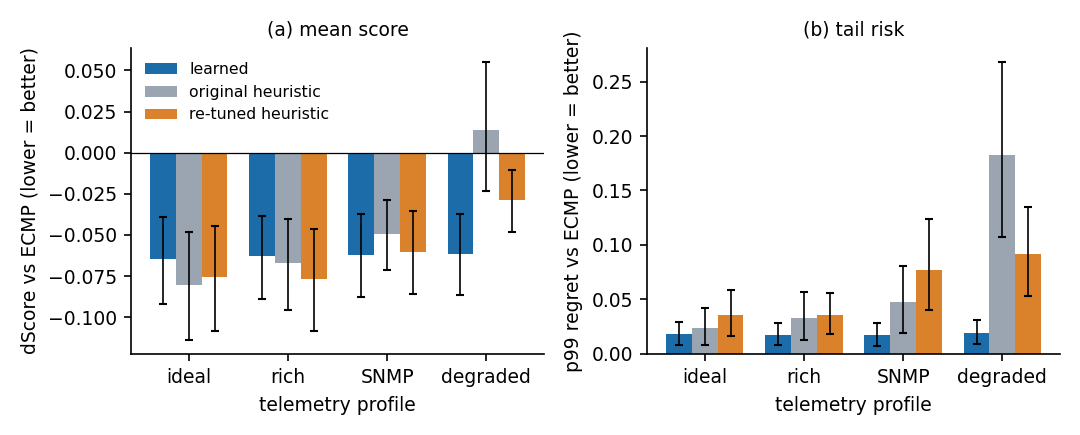
\includegraphics[width=0.8\textwidth]{figures/fig1_zoo.png}
\caption{Held-out Zoo graphs (24): (a) mean dScore and (b) mean per-graph p99 regret, by telemetry profile, for the learned policy (mean of 4 training seeds), the original 40-trial heuristic and the re-tuned heuristic (mean of 5 tuner seeds). Error bars are 95\% bootstrap intervals over graphs; they reflect graph variability, not tuner-seed variability.}
\end{figure*}

Three things change. (1) \textit{Mean performance:}

with the stronger heuristic the learned policy no longer leads under SNMP telemetry (expected diff +0.002 [-0.007, +0.012], 7 wins / 10 ties / 7 losses; the tuner seed with the best tuning score is ahead of the learned policy by 0.010 [-0.023, +0.000]) and trails the heuristic under rich telemetry (-0.014 [-0.027, -0.004]); under ideal telemetry the heuristic stays ahead on average (-0.011, interval includes 0) and with the selected seed (-0.020 [-0.036, -0.008]). The earlier statement that the learned policy wins at SNMP telemetry was partly an artefact of a weakly tuned baseline. (2) \textit{Degraded telemetry:} the learned policy remains ahead (+0.033 [+0.018, +0.049] on average over tuner seeds, 15 wins / 9 ties / 0 losses; +0.021 [+0.010, +0.034] for the selected seed), but by less than against the original heuristic (+0.075). (3) \textit{Tail risk:} the learned policy's mean p99 regret (0.017--0.019) is lower than the re-tuned heuristic's (averaged over tuner seeds 0.036, 0.036, 0.077, 0.092 for ideal, rich, SNMP, degraded). The difference (heuristic minus learned) is +0.018 [+0.000, +0.039] (ideal), +0.018 [+0.004, +0.035] (rich), +0.060 [+0.027, +0.101] (SNMP) and +0.073 [+0.038, +0.113] (degraded), bootstrap over graphs, but the learned policy has the lower p99 on only 9, 10, 13 and 13 of the 24 graphs: the mean difference comes from a minority of graphs on which the heuristic has a large tail, so "lower tail regret" means lower on average, driven by those graphs, and not a uniform advantage. Tuner-seed spread is material (e.g. SNMP dScore from -0.053 to -0.072), so a single tuning run, as used elsewhere in this paper, can move a comparison by about as much as the differences reported. The real-trace comparison, the guard evaluation and the stress scenarios were repeated with the re-tuned heuristic (the seed with the best tuning score per profile, \texttt{configs/tuned\_heuristic\_v2.yaml}; Sections 6.2 and 6.5 and below) and give the same picture; the overload analysis of Section 6.4, the loss-weight sensitivity and the emulation still use the original heuristic. Intervals in this table are bootstrap intervals over graphs (evaluation uncertainty) for a fixed set of trained policies; the spread over tuner seeds is reported separately as the per-seed row and the min-max of the rows, and the two are not combined.

\subsection{Real traces}
Tables: \texttt{experiments/final/table\_real.md} (first run, 4 windows) and \texttt{table\_realw.md} (10 fresh windows). Over the four networks with headroom (Abilene, GEANT, Germany17, Germany50 in the first run; first three in the second), per (network, load) cell, the learned policy (mean of four training seeds) versus the tuned heuristic:

\begin{itemize}
\item first run (12 cells per profile): rich, SNMP-like and degraded telemetry, learned ahead in 12/12 each; clean telemetry 7 learned, 4 tuned, 1 tie;
\item second run (9 cells per profile): rich 8 ahead + 1 tie, SNMP 8 + 1, degraded 9 ahead; clean telemetry 4 learned, 3 tuned, 2 ties. "Ahead" means more than one point of gain.
\item The heuristic falls below ECMP under degraded telemetry on Germany17 (-3\% to -4\%) and, in individual Abilene windows, by up to -51\% (Section 6.4); on GEANT it falls to about 0\% at degraded telemetry on the held-out windows, and on Germany50 it does not collapse.
\item Germany50 (50 nodes, larger than any training graph): learned 33--36\% versus 9--31\%.
\item Brain: gain is about 0.3\% for every method in the 12 windows of the second run; in one window of the first run the learned policy gained 20.9\%, so benefits are confined to rare windows.
\item The oracle gain (n $\le$ 25) is 47--58\% on Abilene and 37\% on Germany17; the zero-shot policy captures roughly half.
\end{itemize}

\textbf{Re-tuned heuristic (primary real-trace evidence).} The tables below this paragraph used the original per-profile heuristic. We recomputed the heuristic column on the same 12 windows per cell with the re-tuned parameters (selected by tuning score, Section 6.1; \texttt{table\_realci\_v2.md}, 36 cells). The paired 95\% interval over windows now excludes zero in favour of the learned policy in 12 cells, in favour of the heuristic in 17 and includes zero in 7. By telemetry profile (learned / heuristic / tie, 9 cells each): ideal 0/9/0, rich 0/6/3, SNMP 3/2/4, degraded 9/0/0. Under degraded telemetry the learned policy is ahead by +7.8 to +13.0 points on every network and load; under ideal telemetry the heuristic is ahead by 2.4--7.7 points. This agrees with the Zoo result of Section 6.1 and replaces the earlier statement that the learned policy leads in 32 of 36 cells, which depended on the weaker heuristic. The window-level evidence below is retained as the record of the original comparison.

\begin{figure}[!t]
\centering
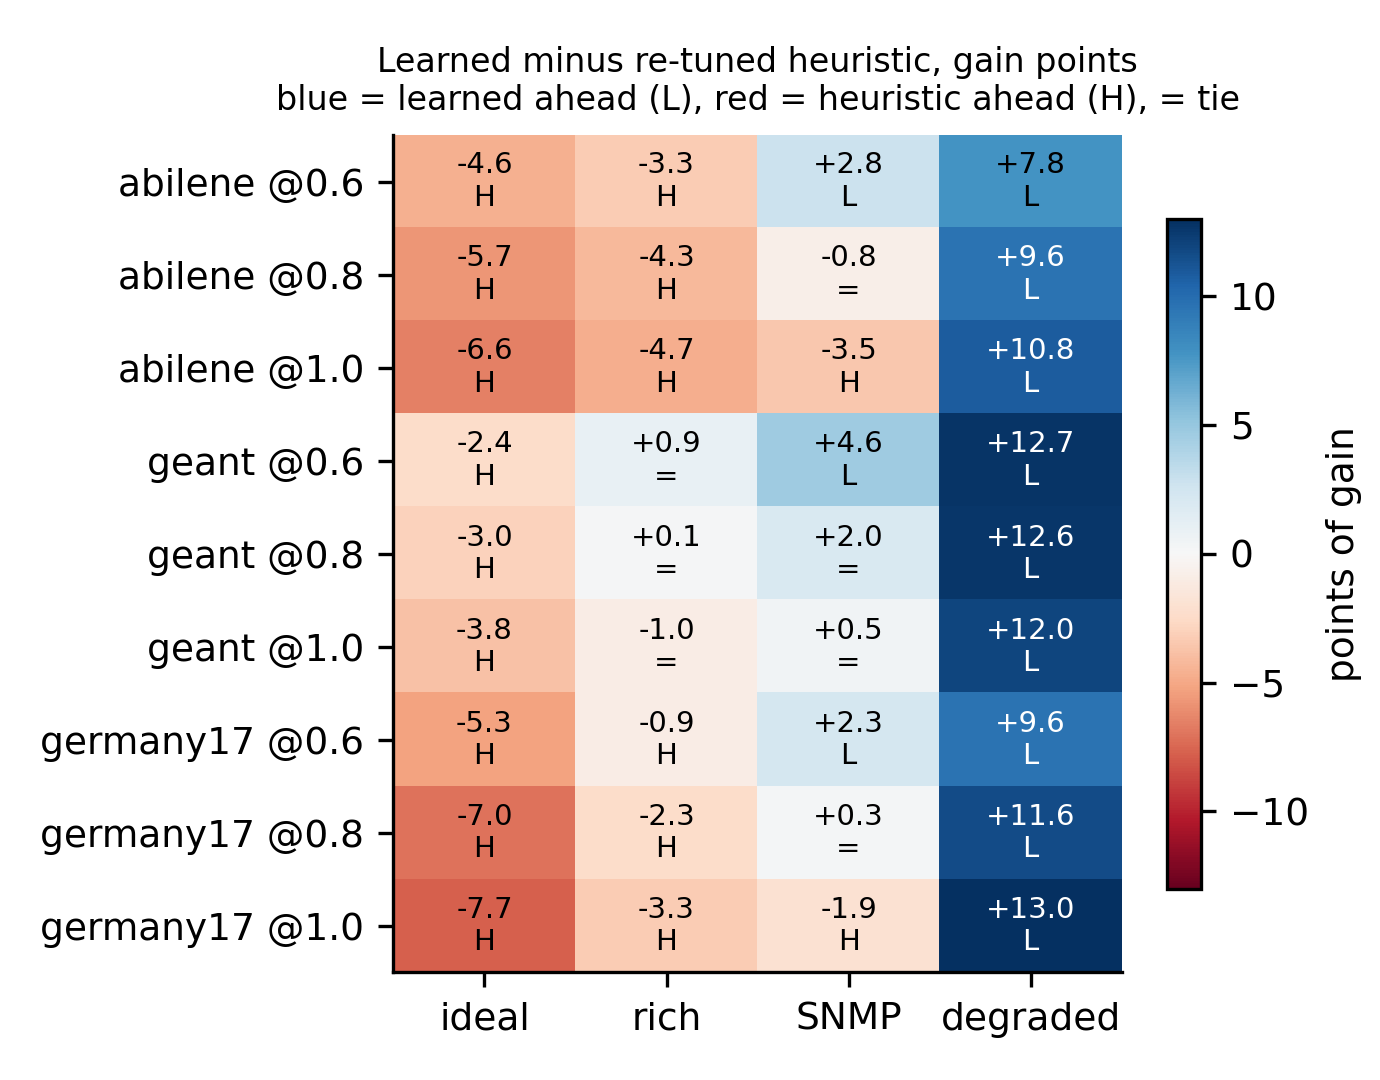
\includegraphics[width=\columnwidth]{figures/fig2_real.png}
\caption{Real traces with the re-tuned heuristic: learned minus heuristic gain in points, per network, load and telemetry profile (12 windows per cell). Letters give the verdict of the paired 95\% bootstrap interval over windows (L learned ahead, H heuristic ahead, = tie).}
\end{figure}

\textbf{Window-level intervals (original heuristic; superseded by the paragraph above).} To report uncertainty consistently we re-ran the real-trace comparison with 12 further independent windows per cell, keeping per-window gains (\texttt{table\_realci.md}; Abilene, GEANT, Germany17; 36 cells; zero-traffic windows skipped). For each cell we bootstrap the paired difference (learned, mean of four training seeds, minus tuned heuristic) over windows. The 95\% interval excludes zero in favour of the learned policy in 32 of 36 cells, in favour of the tuned heuristic in 2 (clean telemetry on Germany17 at loads 0.8 and 1.0, by 2.0 and 4.9 points) and includes zero in 2 (Abilene at load 1.0, clean and SNMP-like telemetry). By telemetry: rich 9/9, degraded 9/9 and SNMP-like 8/9 cells favour the learned policy (rest ties); clean telemetry 6 learned, 2 tuned, 1 tie. Typical differences are +4 to +23 points of gain; under degraded telemetry the heuristic's gain is 13.6--29.3\% on Abilene/GEANT and negative (-5.3 to -6.8\%) on Germany17 while the learned policy stays at 12--45\%. The count for clean telemetry changed between window samples (4/3/2 in the previous run, 6/2/1 here), so clean-telemetry rankings should be read as network- and load-dependent, not as a stable ordering; the non-clean-telemetry result was stable across all three real-trace runs. These windows contain no overloaded windows in the sense of Section 6.4, which are rare.

\subsection{Which impairment drives the ranking, and is it a tuning artefact?}
\textit{Controlled delay experiment} (\texttt{experiments/delay\_controlled.py}, \texttt{table\_delay\_part1.md}): only the delay d varies, everything else is ideal; the tuned heuristic is run with (i) parameters frozen at the values tuned for clean telemetry, (ii) parameters frozen at the values tuned for the degraded profile, and (iii) parameters re-tuned at each d (40-trial random search on four synthetic graphs); the learned policy is the mean of four training seeds. Mean gain \%, load 0.8:

\begin{table*}[!t]
\centering
\scriptsize
\renewcommand{\arraystretch}{1.05}
\adjustbox{max width=\textwidth}{%
\begin{tabular}{lccccc}
\hline
case & d & heuristic, frozen (clean-tuned) & heuristic, frozen (degraded-tuned) & heuristic, re-tuned at d & learned \\
\hline
Abilene & 0 & 34.0 & 16.4 & 41.9 & 34.5 \\
Abilene & 3 & 6.4 & 20.7 & 34.7 & 34.2 \\
Abilene & 5 & 0.0 & 22.5 & 23.2 & 34.5 \\
Abilene & 10 & 0.0 & 0.0 & 21.0 & 34.7 \\
GEANT & 0 & 37.6 & 38.2 & 45.6 & 42.6 \\
GEANT & 3 & 1.9 & 31.9 & 43.6 & 42.5 \\
GEANT & 5 & 0.0 & 24.2 & 23.2 & 42.5 \\
GEANT & 10 & 0.0 & 0.0 & 24.9 & 41.8 \\
Zoo (10 graphs) & 0 & 4.8 & 0.9 & 5.1 & 4.8 \\
Zoo (10 graphs) & 3 & 0.7 & 0.5 & 3.2 & 4.3 \\
Zoo (10 graphs) & 5 & 0.0 & 2.2 & 2.3 & 4.3 \\
Zoo (10 graphs) & 10 & 0.0 & 0.0 & 2.8 & 4.2 \\
\hline
\end{tabular}}
\end{table*}

Two conclusions. First, a heuristic whose parameters are frozen collapses with delay (to about zero at d $\ge$ 5), but this is largely an artefact of mis-tuning: re-tuned at each delay it keeps most of its gain. Second, a re-tuned heuristic matches the learned policy at small delay (d = 3: Abilene 34.7 vs 34.2, GEANT 43.6 vs 42.5, Zoo 3.2 vs 4.3) and is behind at d = 5 and d = 10 in this table (Abilene 23.2 and 21.0 vs about 34.6; GEANT 23.2 and 24.9 vs about 42). The learned policy's gain does not depend on d. The interaction grid below, with repeated tuning, shows the boundary depends on polling period and network. The re-tuning budget is modest (40 trials, synthetic graphs, other impairments ideal), so a stronger tuned baseline might narrow the gap; this is not tested. The per-profile comparisons of Sections 6.1--6.2 use heuristics re-tuned for each profile, so they are not affected by the frozen-parameter artefact.

\textit{Delay $\times$ polling grid with repeated tuning} (\texttt{table\_delay\_repeat.md}; \texttt{experiments/delay\_tuning\_repeat.py}). The first version of this grid used one 40-trial tuning run per cell and was non-monotone in delay (Abilene at P = 20: 33.8, 24.6, 30.0 at d = 0, 3, 10), which we read as tuning noise. We therefore re-tuned the heuristic five times per cell with independent tuner seeds and 80 trials each (same synthetic tuning graphs and objective; the seed with the best \textit{tuning} score is the reported heuristic, so selection never sees the evaluation data). Learned = mean of 4 training seeds. Gain \%, learned minus heuristic, in points ("best seed" is an evaluation-side oracle over the five tuner seeds and therefore favours the heuristic):

\begin{table*}[!t]
\centering
\scriptsize
\renewcommand{\arraystretch}{1.05}
\adjustbox{max width=\textwidth}{%
\begin{tabular}{lccccccccc}
\hline
case & d=0 P=1 & d=0 P=5 & d=0 P=20 & d=3 P=1 & d=3 P=5 & d=3 P=20 & d=10 P=1 & d=10 P=5 & d=10 P=20 \\
\hline
Zoo (10 graphs) & -0.4 & -0.1 & +0.9 & +1.2 & +1.0 & +1.1 & +1.5 & +1.9 & +0.9 \\
Abilene & -7.2 & -2.9 & +5.4 & -2.7 & -1.8 & +8.5 & +3.5 & +6.3 & +6.2 \\
GEANT & -1.7 & +1.8 & +12.5 & +0.7 & +3.8 & +15.5 & +5.0 & +11.3 & +15.0 \\
\hline
\end{tabular}}
\end{table*}

With selection by tuning score the heuristic is ahead in 5 of 18 real-trace cells (Abilene: d $\le$ 3 with P $\le$ 5; GEANT: d = 0, P = 1), within 1 point in two more, and behind in the rest by up to 15.5 points; against the best of five tuner seeds it is ahead in 6 cells and the learned policy is still 2.9--9.5 points ahead in the cells with P = 20 or d = 10 (except one tie), so the large margins are not an artefact of an unlucky tuner run. On Zoo graphs the two are within 0.4 points at d = 0 with P $\le$ 5 and the learned policy is ahead by 0.9--1.9 elsewhere. The learned policy's gain varies by under 2 points across the grid, while the heuristic's decreases with both delay and polling period (Abilene, selected seed: 41.7 at d = 0, P = 1 down to 27.8 at d = 10, P = 20). The tuner-seed range inside a cell is up to about 10 points (e.g. GEANT d = 10, P = 1: 24.4--36.8), so single-cell margins below that size should not be over-interpreted; the pattern across cells is what we report. This is a gradient, not a sharp threshold: there is no delay value at which the ranking flips independent of polling period and network. The experiment has no window-level confidence intervals, and tuning uses 4 synthetic graphs, so a stronger or in-domain search could shift the boundary; the single-run grid (\texttt{table\_delay\_part2.md}) is retained as raw data but superseded by this table.

\textit{Window-level intervals for the grid} (\texttt{table\_delay\_ci.md}; \texttt{experiments/delay\_grid\_ci.py}). For Abilene and GEANT the heuristic selected above is evaluated on 16 fresh windows per cell (seeds not used in tuning or in the tables above; 14 windows remain on GEANT after skipping zero-traffic ones), paired with the mean of four learned training seeds; bootstrap 95\% interval over windows of learned minus heuristic gain (points); verdict L = learned ahead, H = heuristic ahead, = tie:

\begin{table*}[!t]
\centering
\scriptsize
\renewcommand{\arraystretch}{1.05}
\adjustbox{max width=\textwidth}{%
\begin{tabular}{lccccccc}
\hline
network & d & P & heuristic \% & learned \% & diff [95\% CI] & verdict & windows \\
\hline
abilene & 0 & 1 & 44.9 & 30.9 & -14.0 [-27.8, -5.6] & H & 16 \\
abilene & 0 & 5 & 40.8 & 30.6 & -10.3 [-25.9, -0.3] & H & 16 \\
abilene & 0 & 20 & 38.2 & 32.0 & -6.2 [-21.8, +2.9] & = & 16 \\
abilene & 3 & 1 & 42.6 & 31.2 & -11.4 [-26.8, -1.8] & H & 16 \\
abilene & 3 & 5 & 40.9 & 28.6 & -12.3 [-29.4, +0.4] & = & 16 \\
abilene & 3 & 20 & 35.8 & 29.8 & -6.0 [-22.7, +5.8] & = & 16 \\
abilene & 10 & 1 & 37.0 & 31.8 & -5.1 [-22.4, +5.0] & = & 16 \\
abilene & 10 & 5 & 37.4 & 31.7 & -5.7 [-21.3, +4.0] & = & 16 \\
abilene & 10 & 20 & 32.8 & 29.8 & -3.0 [-18.7, +7.0] & = & 16 \\
geant & 0 & 1 & 38.5 & 34.4 & -4.1 [-5.2, -3.0] & H & 14 \\
geant & 0 & 5 & 33.9 & 34.2 & +0.4 [-1.1, +1.9] & = & 14 \\
geant & 0 & 20 & 22.2 & 32.9 & +10.7 [+8.3, +12.8] & L & 14 \\
geant & 3 & 1 & 33.8 & 34.3 & +0.5 [-1.6, +2.9] & = & 14 \\
geant & 3 & 5 & 31.7 & 34.2 & +2.5 [+1.0, +4.2] & L & 14 \\
geant & 3 & 20 & 20.4 & 32.7 & +12.3 [+9.3, +15.0] & L & 14 \\
geant & 10 & 1 & 29.5 & 33.2 & +3.7 [+1.1, +6.4] & L & 14 \\
geant & 10 & 5 & 23.6 & 32.9 & +9.2 [+7.3, +10.9] & L & 14 \\
geant & 10 & 20 & 20.5 & 31.4 & +10.9 [+7.9, +13.5] & L & 14 \\
\hline
\end{tabular}}
\end{table*}

\begin{figure*}[!t]
\centering
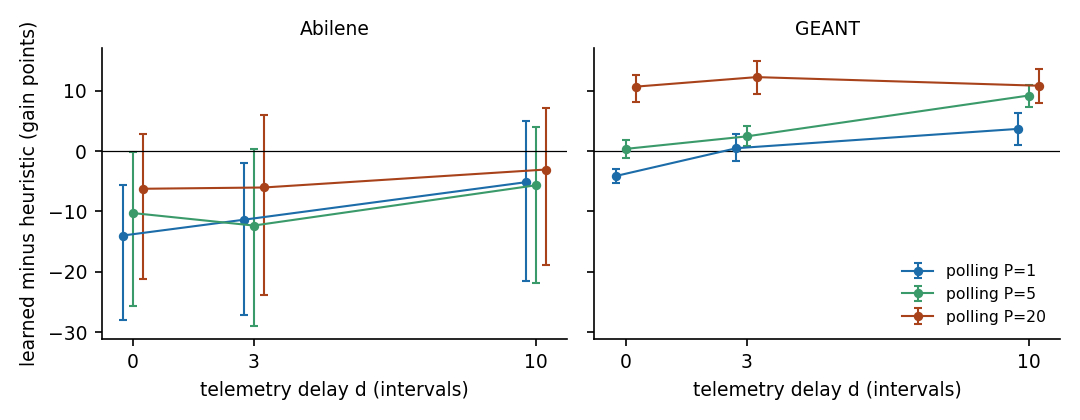
\includegraphics[width=0.8\textwidth]{figures/fig3_delay.png}
\caption{Delay $\times$ polling grid with the re-tuned heuristic (best tuning score of 5 tuner seeds): learned minus heuristic gain in points on 16 fresh windows per cell, with 95\% bootstrap intervals over windows. Abilene intervals mostly include zero; on GEANT the learned policy's advantage grows with delay and polling period.}
\end{figure*}

On GEANT the pattern is clear: the heuristic is ahead only at d = 0, P = 1 (-4.1 [-5.2, -3.0]), two cells are ties, and the learned policy is ahead in the other six, by 2.5--12.3 points; its advantage grows with delay and polling period. On Abilene the picture is \textbf{not} resolved: the point estimate favours the heuristic in all nine cells, by 3.0--14.0 points, the interval excludes zero (heuristic ahead) in three cells and includes zero in six, and the window-to-window spread is large (interval half-widths of 10--15 points). This contradicts the earlier Abilene point estimates (learned ahead by 5--8 points at P = 20 or d = 10, from a different sample of 6 windows without intervals), so the Abilene "learned advantage at high staleness" in the preceding table is window-sample dependent and not an established result. It is also in tension with the profile-level real-trace results of Section 6.2 (learned ahead on Abilene under degraded telemetry in a 12-window sample with a heuristic tuned per profile); both samples are small, and we cannot say from this evidence how much of the Abilene difference is window sampling and how much is heuristic tuning. The tuner saw only synthetic graphs, never a real trace or evaluation window.

\textit{Audit of the Abilene discrepancy} (\texttt{table\_abilene\_audit.md}; \texttt{experiments/abilene\_audit.py}). Both experiments use the same four model checkpoints, the same trace loader and scaling, the same gain definition (1 - max-util / ECMP max-util), the same environment and horizon, and random 100-interval windows chosen by seed; they differ in the window sample (seeds 20000+, 12 windows, versus 15000+, 16 windows), the telemetry (named profiles with noise and drops versus clean delay/polling) and the heuristic parameters (per-profile, 40 trials, one run, versus best-of-5 80-trial). We evaluated both heuristic parameter sets under the same telemetry on both window samples (load 0.8, learned minus heuristic, points, bootstrap 95\% over windows):

\begin{table*}[!t]
\centering
\scriptsize
\renewcommand{\arraystretch}{1.05}
\adjustbox{max width=\textwidth}{%
\begin{tabular}{lccccc}
\hline
telemetry & window set & heuristic params & heuristic \% & learned \% & learned - heuristic [95\% CI over windows] \\
\hline
snmp & A (20000+, 12 windows) & yaml (per-profile, 40 trials) & 27.9 & 36.3 & +8.4 [+4.2, +12.3] \\
snmp & A (20000+, 12 windows) & grid best-of-5 (d=3,P=5) & 17.7 & 36.3 & +18.6 [+5.7, +32.0] \\
snmp & B (15000+, 16 windows) & yaml (per-profile, 40 trials) & 32.7 & 31.4 & -1.3 [-18.5, +9.9] \\
snmp & B (15000+, 16 windows) & grid best-of-5 (d=3,P=5) & 29.3 & 31.4 & +2.1 [-16.0, +15.0] \\
degraded & A (20000+, 12 windows) & yaml (per-profile, 40 trials) & 17.0 & 36.1 & +19.1 [+9.0, +30.2] \\
degraded & A (20000+, 12 windows) & grid best-of-5 (d=3,P=5) & 31.2 & 36.1 & +4.9 [+1.3, +9.0] \\
degraded & B (15000+, 16 windows) & yaml (per-profile, 40 trials) & 24.2 & 28.6 & +4.5 [-14.3, +19.0] \\
degraded & B (15000+, 16 windows) & grid best-of-5 (d=3,P=5) & 35.5 & 28.6 & -6.8 [-23.6, +5.6] \\
clean d=3,P=5 & A (20000+, 12 windows) & grid best-of-5 (d=3,P=5) & 37.0 & 36.6 & -0.4 [-2.5, +1.8] \\
clean d=3,P=5 & B (15000+, 16 windows) & grid best-of-5 (d=3,P=5) & 40.9 & 28.6 & -12.3 [-31.9, +0.3] \\
\hline
\end{tabular}}
\end{table*}

Two sources of variation are visible. (1) \textit{Window sample:} with identical policies and telemetry (clean, d = 3, P = 5) the learned policy is level with the heuristic on set A (-0.4 [-2.5, +1.8]) and 12.3 points behind on set B, and under the SNMP profile with the same parameters the difference moves from +8.4 [+4.2, +12.3] on A to -1.3 [-18.5, +9.9] on B; the learned policy's own gain moves from 36 to 29--31\%. (2) \textit{Heuristic parameters:} under the degraded profile the grid-selected parameters reach 31.2\% on A against 17.0\% for the per-profile parameters, so the profile-level advantage of the learned policy on Abilene partly reflects a weakly tuned baseline in that table. We found no inconsistency in implementation or preprocessing, and we cannot attribute the remaining discrepancy beyond these two sources. Abilene conclusions are therefore limited to "the sign depends on the window sample and on the heuristic's tuning"; the Section 6.2 per-profile Abilene results should be read with this caveat.

\textit{One-at-a-time sweep with frozen parameters} (\texttt{table\_telemetry\_sweep.md}; heuristic parameters are those tuned for the nearest standard profile, so the collapse is exaggerated as described above; 10 Zoo graphs with n $\le$ 25, Abilene and GEANT at load 0.8; mean gain \%, tuned / learned):

\begin{table}[!t]
\centering
\footnotesize
\renewcommand{\arraystretch}{1.05}
\adjustbox{max width=\columnwidth}{%
\begin{tabular}{llll}
\hline
parameter (range) & Zoo & Abilene & GEANT \\
\hline
delay d: 0 $\rightarrow$ 10 intervals & 5.2 $\rightarrow$ 0.0 / 4.6 $\rightarrow$ 4.0 & 35.0 $\rightarrow$ 0.3 / 29.7 $\rightarrow$ 31.7 & 23.5 $\rightarrow$ 0.0 / 25.4 $\rightarrow$ 26.2 \\
polling period P: 1 $\rightarrow$ 20 & 5.2 $\rightarrow$ -2.2 / 4.6 $\rightarrow$ 4.2 & 35.0 $\rightarrow$ 22.1 (17.8 at P=10) / 29.7 $\rightarrow$ 27.7 & 23.5 $\rightarrow$ 16.1 / 25.4 $\rightarrow$ 25.8 \\
noise sigma: 0 $\rightarrow$ 0.4 & 5.2 $\rightarrow$ 1.6 / 4.6 $\rightarrow$ 4.2 & 35.0 $\rightarrow$ 29.1 / 29.7 $\rightarrow$ 29.0 & 23.5 $\rightarrow$ 30.0 / 25.4 $\rightarrow$ 22.2 \\
missing counters p: 0 $\rightarrow$ 0.4 & 5.2 $\rightarrow$ 3.9 / 4.6 $\rightarrow$ 4.6 & 35.0 $\rightarrow$ 35.9 / 29.7 $\rightarrow$ 27.5 & 23.5 $\rightarrow$ 24.1 / 25.4 $\rightarrow$ 25.4 \\
\hline
\end{tabular}}
\end{table}

Delay and polling period (the staleness parameters) change the ranking most; noise and missing counters have little effect, and on the real traces the heuristic even gains from moderate noise (smoothing; its parameters switch to the SNMP/rich profile settings at those points). Read the delay row together with the controlled experiment above.

Rule-install latency L (0 $\rightarrow$ 8 intervals, \texttt{table\_install\_latency.md}, same setup, tuned / learned gain \%): Zoo 3.8 $\rightarrow$ 1.9 / 3.5 $\rightarrow$ 3.0; Abilene 40.8 $\rightarrow$ 37.1 / 33.6 $\rightarrow$ 32.1 (tuned p99 regret -0.03 $\rightarrow$ +0.84); GEANT 33.0 $\rightarrow$ 31.2 / 34.8 $\rightarrow$ 31.4. Install latency hurts the reactive heuristic's tail more than its mean, and matters much less than telemetry delay; on these Abilene windows the tuned heuristic with ideal telemetry is ahead of the learned policy, consistent with Section 6.2.

\subsection{Sensitivity to the load-scaling rule}
Scaling each real trace so that the \textit{mean} or the 95th percentile (instead of the median) of the ECMP max-utilisation equals 0.8 (\texttt{table\_scaling.md}; Abilene, GEANT, Germany17; ideal and degraded telemetry; 6 windows; 18 cells): learned ahead in 12, tuned ahead in 4 (clean telemetry on Abilene and Germany17, and Abilene at the 95th percentile with degraded telemetry), 2 ties; under degraded telemetry the learned policy is ahead in 8 of 9 cells. The conclusion does not depend on the scaling rule; the absolute numbers do.

\subsection{What carries the result: baselines and ablations}
Held-out windows (last 30\% of the trace), gain \% (\texttt{experiments/final/table\_ft.md}; seed-0 GNN):

\begin{table*}[!t]
\centering
\scriptsize
\renewcommand{\arraystretch}{1.05}
\adjustbox{max width=\textwidth}{%
\begin{tabular}{lccccc}
\hline
Abilene @0.8 & tuned & static LP & DOTE-style (degraded-trained) & GNN zero-shot & GNN fine-tuned \\
\hline
ideal & 33.6 & 34.5 & 49.1 & 23.7 & 46.2 \\
SNMP & 27.7 & 34.5 & 49.1 & 22.4 & 41.3 \\
degraded & 23.5 & 34.5 & 48.9 & 22.5 & 39.3 \\
\hline
\end{tabular}}
\end{table*}

On GEANT the DOTE-style model reaches about 18\% in every profile, the zero-shot policy 15--18\%, the fine-tuned policy 16--19\% and static LP -38.6\% (traffic is not stationary). Hence: (a) with per-network history a DOTE-style model beats the zero-shot GNN, and fine-tuning recovers most of the difference on Abilene but little on GEANT; (b) robustness to telemetry is a property of any policy that does not rely on fresh counters, not specific to our GNN; (c) what the zero-shot policy offers is no need for per-network training data. Ablations (24 Zoo graphs; \texttt{table\_ablations.md}, one seed, and \texttt{table\_gnn\_vs\_mlp.md}, four training seeds each for the full model, the per-link MLP and the no-fluid-feature model): removing history costs +0.003 at ideal telemetry only; removing the age input is $\sim$0. \textbf{Matched-seed GNN vs MLP:} the per-link MLP (no message passing) has mean dScore -0.068 (ideal) / -0.063 (degraded) against -0.065 / -0.061 for the full graph model; seed-averaged paired difference -0.0031 [-0.0054, -0.0011] and -0.0020 [-0.0040, -0.0002], the MLP better on 14 of 24 graphs in both profiles. Its p99 regret is slightly worse under degraded telemetry (0.022 vs 0.019). So message passing does not help; the effect sizes are small and we claim only "no benefit", not that MLPs are better. \textbf{Fluid-model features:} removing them costs +0.0082 [+0.0048, +0.0121] (ideal) and +0.0144 [+0.0085, +0.0206] (degraded) and worsens p99 regret (0.018 to 0.029 degraded); the full model is better on 21--22 of 24 graphs. The model-based features, not the graph architecture, carry the result. Training with randomised telemetry versus ideal-only: the mean differences are within seed noise ($\sim$0.002), but the randomised model has a lower p99 regret under degraded telemetry (0.019 vs 0.027 over four seeds).

\subsection{Where it fails: overload}
Real-trace windows in which ECMP's own mean max-utilisation exceeds 2 (traffic surges far above the requested load) lie outside the training range (loads 0.5--1.1). On Abilene at load 0.8 over 30 windows: in 27 typical windows the learned policy has median gain 36.5\% and is never worse than ECMP, while the tuned heuristic has median 31.5\% (worst window -50.8\% under degraded telemetry); in 3 overloaded windows the tuned heuristic gains 45--49\% and the learned policy 9--21\% (worse than ECMP in one of three; worst case +3 to +7 in absolute max-util). The guard lifts the learned policy to 20--27\% in those windows (\texttt{table\_overload.md}). Tail statistics pooled over windows are therefore dominated by a few surges. Repeated with the re-tuned heuristic (\texttt{table\_overload\_v2.md}, same 30 windows): typical windows, ideal telemetry, heuristic median gain 41.1\% (worst 8.6\%) vs learned 36.5\% (worst 2.1\%); degraded telemetry, heuristic 28.6\% (worst -21.5\%) vs learned 35.3\% (worst +1.4\%, never below ECMP); overloaded windows (3), heuristic 49.0\% (ideal) and 42.5\% (degraded) vs learned 9.1\% and 20.8\%, lifted by the guard to 19.9\% and 26.8\%. The qualitative picture is unchanged: the heuristic is better on average with ideal telemetry and in overloaded windows, the learned policy is better and safer under degraded telemetry.

\subsection{Guard}
Definitions (per interval, using the true demand, simulator only): \textit{beneficial} proposal = true max-util below 0.99 $\times$ ECMP's, \textit{harmful} = above 1.01 x; false rejection = beneficial proposals among fallbacks; harm caught = harmful proposals replaced. Zoo graphs (10 graphs with n $\le$ 25, \texttt{table\_guard\_audit.md}), headline guard (L2 only, eps = -0.06):

\begin{table*}[!t]
\centering
\scriptsize
\renewcommand{\arraystretch}{1.05}
\adjustbox{max width=\textwidth}{%
\begin{tabular}{lccccc}
\hline
scenario & fallback & false rejection & harm caught & gain kept & p99 regret raw $\rightarrow$ guarded \\
\hline
ideal & 71\% & 12\% & 43\% & 83\% & +0.050 $\rightarrow$ +0.019 \\
degraded & 72\% & 14\% & 22\% & 76\% & +0.065 $\rightarrow$ +0.057 \\
link failure, degraded & 80\% & 13\% & 90\% & 91\% & +0.148 $\rightarrow$ +0.021 \\
demand shift, degraded & 73\% & 18\% & 53\% & 74\% & +0.084 $\rightarrow$ +0.058 \\
\hline
\end{tabular}}
\end{table*}

On real Abilene and GEANT traces (load 0.8, three typical windows each) the guard fires in only 0--2\% of intervals because the learned policy's proposals are essentially never harmful there (0.0\% of accepted intervals harmful; raw p99 regret already $\le$ 0); its value on real traces appears in overloaded windows (Section 6.4) and for the tuned heuristic. On the 24 test graphs the per-graph p99 regret falls from 0.019 to 0.008 at degraded telemetry (average of per-graph p99), while the pooled p99 above falls only from +0.065 to +0.057: the guard cuts the typical tail but misses harmful proposals concentrated in a few graphs. The guard is most effective under link failures. It falls back often (71--80\%) yet keeps 74--91\% of the gain because fallback occurs mostly in low-gain intervals. For the tuned heuristic under degraded telemetry the guard improves the gain by 2.3 points on real traces and lowers its p99 regret from 0.198 to 0.074; the validation-chosen guard barely affects the learned policy on real traces (0.0--0.8 points).

\textbf{Guard against the re-tuned heuristic} (\texttt{table\_v2\_guard\_stress.md}; 24 Zoo graphs, L2-only guard, eps = -0.06; mean dScore, p99 regret):

\begin{table}[!t]
\centering
\scriptsize
\renewcommand{\arraystretch}{1.05}
\adjustbox{max width=\columnwidth}{%
\begin{tabular}{lcccc}
\hline
telemetry & learned & learned + guard & re-tuned heuristic & heuristic + guard \\
\hline
ideal & -0.064, 0.017 & -0.054, 0.008 & -0.085, 0.026 & -0.064, 0.008 \\
rich & -0.062, 0.018 & -0.051, 0.009 & -0.073, 0.041 & -0.058, 0.019 \\
SNMP & -0.062, 0.017 & -0.051, 0.010 & -0.072, 0.056 & -0.054, 0.031 \\
degraded & -0.060, 0.019 & -0.049, 0.008 & -0.040, 0.093 & -0.042, 0.030 \\
\hline
\end{tabular}}
\end{table}

The guard roughly halves the p99 regret of both policies (learned 0.017--0.019 to 0.008--0.010; heuristic 0.026--0.093 to 0.008--0.031) and its fallback rate is 78--84\%. Its cost in average dScore is about +0.011 for the learned policy in every profile and +0.015 to +0.021 for the heuristic at ideal, rich and SNMP telemetry, but essentially nothing for the heuristic under degraded telemetry (-0.040 to -0.042), where it lowers p99 regret from 0.093 to 0.030. With the guard, the learned policy and the re-tuned heuristic have similar p99 regret at ideal and rich telemetry (0.008 vs 0.008, 0.009 vs 0.019) and the learned policy is lower elsewhere. The guard is therefore a tail-risk trade against mean performance for either policy, not a property that favours the learned one.

\subsection{Operational cost and emulation}
Without a rate limiter the learned policy updates 91\% of demands every interval in simulation (Zoo, ideal telemetry); a 5\% threshold cuts this to 8\% and a 10\% threshold to 2.4\% with unchanged gain (3.1\%) (\texttt{table\_ratelimit.md}); the tuned heuristic already updates about 2.5\% of demands. On the real traces (\texttt{table\_ratelimit\_real.md}, degraded telemetry) the learned policy updates 98.5\% (Abilene) and 100\% (GEANT) of demands per interval without a limiter; thresholds of 5\%, 10\% and 20\% cut this to 5.1/1.7/0.9\% (Abilene) and 6.3/1.9/0.8\% (GEANT) while the gain stays or rises (Abilene 26.4 $\rightarrow$ 27.6/32.4/36.8\%, GEANT 37.9 $\rightarrow$ 38.2/38.5/37.7\%; thresholds of 0.5 lose gain). The threshold also damps oscillation, so the update-rate cost is largely avoidable in simulation.

Emulation: Mininet with Open vSwitch and a Ryu controller reading real OpenFlow counters, 24 flows, four scenarios (three traffic seeds on a 10-node graph, one 12-node random graph), six policy/telemetry runs each plus a run with a 20\% update threshold (\texttt{table\_emu2.md}, controller with the fail-safe fixes, 28 runs). Simulator and emulator agree: across the 24 runs at the default 5\% threshold the correlation between emulated and simulated mean max-utilisation is 0.99, the mean absolute difference 0.017 and the bias +0.010; per-run time-series correlation is 0.83--0.98; the policy ranking agrees (Kendall tau 0.47--0.73 per scenario). Means over the four scenarios (emulated max-util / flow-mods per minute / control loop):

\begin{table}[!t]
\centering
\footnotesize
\renewcommand{\arraystretch}{1.05}
\adjustbox{max width=\columnwidth}{%
\begin{tabular}{llll}
\hline
policy [telemetry] & max-util & flow-mods/min & loop ms \\
\hline
ECMP & 0.866 & 0 & 9 \\
original tuned heuristic [SNMP] & 0.798 & 33 & 9 \\
original tuned heuristic [degraded] & 0.808 & 30 & 9 \\
re-tuned heuristic [SNMP] & 0.772 & 140 & 14 \\
re-tuned heuristic [degraded] & 0.806 & 139 & 14 \\
learned [SNMP] & 0.763 & 270 & 12 \\
learned [degraded] & 0.772 & 332 & 14 \\
learned [degraded], threshold 0.2 & 0.790 & 76 & 12 \\
learned + guard (L2, eps -0.06) [degraded] & 0.794 & 258 & 12 \\
\hline
\end{tabular}}
\end{table}

The re-tuned heuristic rows come from a re-run of the same four scenarios (\texttt{table\_emu3.md}, 8 runs; sim-vs-emu correlation 1.00, mean |emu - sim| 0.018). The re-tuned heuristic is much better than the original one under SNMP telemetry (0.772 vs 0.798, close to the learned policy's 0.763) but reprograms about 140 flows per minute instead of 30, so the learned policy reprograms about two times more flows than the re-tuned heuristic (270--332 vs 139), not ten times. Under degraded telemetry the learned policy is ahead (0.772 vs 0.806, loss 0.0080 vs 0.0095) in all four scenarios (by only 0.001 in emu10\_s0); under SNMP the two are level on average (per scenario the learned policy is lower in three and higher in one). A 20\% update threshold cuts the learned policy's updates 4.4-fold (332 to 76 per minute) at a cost of 0.018 in max-util, leaving it ahead of the re-tuned heuristic under degraded telemetry (0.790 vs 0.806). In the emulator the guard costs more than in simulation (0.794 vs 0.772 max-util, and packet loss 0.0143 vs 0.0080 against the unguarded policy). Loop times were measured with the host otherwise idle; capacities are scaled down and traffic is synthetic, so absolute rates do not transfer.

Decision latency (single CPU thread, p50 / p99 over 100 intervals, \texttt{table\_latency.md}): the learned policy takes 2.1 / 4.4 ms on a 12-node graph (132 demands), 11.8 / 19.7 ms at 25 nodes (600 demands), 84 / 114 ms at 50 nodes (2,450 demands) and 311 / 412 ms at 80 nodes (6,320 demands), against 0.3 to 23 ms for the tuned heuristic; Brain (161 nodes, 600 demands) takes 31 ms. Cost grows roughly with links $\times$ demands, which is fine for minute-scale control intervals but not for sub-second loops on networks above about 50 nodes with all-pairs demands.

\subsection{Audit tool}
Run on four real networks with degraded telemetry (polling every 5 intervals, delay 3, noise 0.2, loss 0.1; 6 trace windows; \texttt{reports/*.html}), using the re-tuned heuristic. Abilene: use the tuned heuristic (30.6\%, 95\% interval [27.2, 34.1]; best-case headroom 56.5\%), not distinguishable from the learned policy or its guarded version on these six windows; GEANT: use the learned policy (37.5\% [23.1, 51.0]), with a warning that the heuristic is worse than ECMP in 7\% of intervals and that no method keeps p99 regret under 0.02; Germany50: use the learned policy (33.9\% [30.7, 36.8]), not distinguishable from its guarded version; Brain: stay on ECMP, flagged provisional because six windows cannot rule out the rare surge window in which the learned policy gained 21\%. With the original heuristic the Abilene and GEANT recommendations were the opposite (learned and guarded heuristic respectively; \texttt{reports/v1\_original\_heuristic/}): with six windows and a close call, the recommendation depends on the heuristic's tuning, which is the paper's own point and a reason to run the tool on more windows. The tool therefore reports intervals and ties, not only a winner, and says when the sample is too small. It remains an offline estimate; its verdicts have not been validated against any operator decision.

\section{Negative results}
LP-teacher distillation (DAgger) produced a weak student (6.4\% gain vs 15.0\% for the tuned heuristic on training graphs); PPO fine-tuning did not change it; direct optimisation through the fluid model fixed this. Randomised-telemetry training did not improve mean performance over ideal-only training. A per-link MLP did as well as the GNN, with four matched seeds each (Section 6.3). Static LP routing is excellent on a stationary network (Abilene) and disastrous on a non-stationary one (GEANT).

\section{Limitations and status of claims}
\begin{itemize}
\item Fluid model: no TCP, queueing or packet dynamics. The guard offers no formal guarantee; it is an empirically evaluated filter and misses most harmful proposals under degraded telemetry on Zoo graphs.
\item Real traffic but scaled to a target load by factors from 0.02 to 23 (Section 3); trace capacities for Germany17/50 are not meaningful in absolute terms; some traces contain extreme outlier intervals. The conclusion is insensitive to the scaling rule (6.2b), the absolute numbers are not. Capacities are the networks' published module sizes where available.
\item Telemetry faults are modelled, not measured on a deployed network.
\item Four training seeds (not ten); ablations, DOTE-style and fine-tuned models have one seed; evaluation seeds 4--12 (not 20).
\item DOTE-style and fine-tuned models need per-network history; only Abilene and GEANT have enough.
\item Germany17 and Germany50 have one day of data; their windows overlap.
\item Out-of-range overload hurts the zero-shot policy (6.4).
\item No comparison with Teal or other published systems (Teal's full text was read: it optimises total flow or MLU against LP/NCFlow/POP baselines with accurate demand inputs and treats staleness only as solver run time, so it is not a like-for-like baseline for telemetry impairments); DOTE-style is our re-implementation of the idea, not the authors' code.
\item The heuristic's tuning budget is 80 trials per tuner seed on four synthetic graphs; spread over five tuner seeds is up to $\sim$0.02 dScore on Zoo and $\sim$10 points of gain in the delay grid, so single-run comparisons are fragile. The overload (6.4), loss-weight and emulation results use the original 40-trial heuristic and were not repeated. The in-domain tuning of the heuristic on a network's own history (which the learned policy's fine-tuning variants receive) was not tested.
\item Not claimed: a general performance win; being first to show degradation under delay (LOGGIA); production readiness.
\end{itemize}

\section{Reproducibility and availability}
Code, configuration, trained policies and result tables are in the project repository. \textbf{Repository URL and commit hash: [to be added by the authors at submission; the repository is currently local only, with no public remote].} Environment: Python 3.9+ (tested 3.13, Windows 11 and the Docker images), \texttt{pip install -e ".[dev,rl]"} (torch CPU), \texttt{python -m pytest -q} (39 tests). Data: the SNDlib matrices are public (sndlib.put.poznan.pl; Abilene, GEANT, Germany17/50, Brain) and are \textit{not} redistributed in the repository; they are downloaded and prepared with \texttt{python -m stale\_but\_safe.env.real prepare}. Topology Zoo graphs are bundled under their original licence terms (to be checked for redistribution before release). Each table has one script in \texttt{experiments/} (listed in \texttt{README.md}, with job queues in \texttt{runs/*.sh}); seeds, window selection (random 100-interval windows by integer seed), tuner seeds (100--104), the model-selection rule (heuristic: best tuning score on four synthetic graphs; learned: fixed training schedule, no selection on test data) and the bootstrap procedures (percentile, 4000 resamples, fixed seed) are in the scripts and Section 5. Emulation (Docker, Mininet, Ryu) is described in \texttt{docs/howto.md} and needs an otherwise idle machine because it runs in real time. A clean-environment reproduction check is recorded in \texttt{docs/reproduction\_check.md}.

\section*{Acknowledgment: Use of AI Tools}
In accordance with IEEE policy, the use of generative AI is disclosed here. An AI coding assistant (Claude Code, Anthropic; Claude Sonnet 5.5 and earlier Claude models) generated or substantially produced the simulator, training, evaluation, audit-tool and emulation code, the experiment scripts and analysis, the figures, and the drafting and revision of the text of every section of this manuscript. The research questions, the choice of venue, and the decisions to retract or narrow claims in response to review comments were made by the author, who is responsible for the content of the article. The assistant is not an author. [Before submission the author must review this statement and the whole manuscript, and confirm that his institution's policy permits AI-assisted work.]

\begin{thebibliography}{99}
\bibitem{r1} Y. Perry, F. V. Frujeri, C. Hoch, S. Kandula, I. Menache, M. Schapira, A. Tamar. DOTE: Rethinking (Predictive) WAN Traffic Engineering. \textit{NSDI}, 2023, pp. 1557--1581. arXiv:2303.00735.
\bibitem{r2} Z. Xu, F. Y. Yan, R. Singh, J. T. Chiu, A. M. Rush, M. Yu. Teal: Learning-Accelerated Optimization of WAN Traffic Engineering. \textit{ACM SIGCOMM}, 2023, pp. 378--393. doi:10.1145/3603269.3604857; arXiv:2210.13763.
\bibitem{r3} J. Zhang, M. Ye, Z. Guo, C.-Y. Yen, H. J. Chao. CFR-RL: Traffic Engineering with Reinforcement Learning in SDN. \textit{IEEE JSAC} 38(10), 2020, pp. 2249--2259. doi:10.1109/JSAC.2020.3000371.
\bibitem{r4} A. Boltres, N. Freymuth, B. Schichtholz, M. Koenig, G. Neumann. Towards Near-Real-Time Telemetry-Aware Routing with Neural Routing Algorithms. \textit{TMLR}, 2026. arXiv:2604.02927.
\bibitem{r5} W. Jia, J. Wang, Z. Yan, T. Liu, Y. Ren, K. Lei. EnvelopeTC: Hierarchical Intra-Path Learning for Adaptive Traffic Control. \textit{IEEE JCC}, 2026. doi:10.1109/JCC72984.2026.00071; arXiv:2605.09473.
\bibitem{r6} F. Gui, S. Wang, D. Li, L. Chen, K. Gao, C. Min, Y. Wang. RedTE: Mitigating Subsecond Traffic Bursts with Real-time and Distributed Traffic Engineering. \textit{ACM SIGCOMM}, 2024. doi:10.1145/3651890.3672231.
\bibitem{r7} H. Mao, M. Schwarzkopf, H. He, M. Alizadeh. Towards Safe Online Reinforcement Learning in Computer Systems ("Training Wheels"). \textit{NeurIPS 2019} (workshop paper; the PDF footer names the 33rd NeurIPS, Vancouver).
\bibitem{r8} M. Ye, J. Zhang, Z. Guo, H. J. Chao. FlexDATE: Flexible and Disturbance-Aware Traffic Engineering with Reinforcement Learning in Software-Defined Networks. \textit{IEEE/ACM Trans. Networking}, 2022 (online; issue 2023). doi:10.1109/TNET.2022.3217083.
\bibitem{r9} M. Ye, J. Zhang, Z. Guo, H. J. Chao. Roracle: Enabling Lookahead Routing for Scalable Traffic Engineering with Supervised Learning. \textit{IEEE ICNP}, 2023. doi:10.1109/ICNP59255.2023.10355645.
\bibitem{r10} X. Liu, S. Zhao, Y. Cui, X. Wang. FIGRET: Fine-Grained Robustness-Enhanced Traffic Engineering. \textit{ACM SIGCOMM}, 2024. arXiv:2405.04932.
\bibitem{r11} M. Ye, J. Zhang, Z. Guo, H. J. Chao. DATE: Disturbance-Aware Traffic Engineering with Reinforcement Learning in Software-Defined Networks. \textit{IEEE/ACM IWQoS}, 2021. doi:10.1109/IWQOS52092.2021.9521343. (Located 2026--10--14 via the authors' publication page; the paper itself has not been opened, so it is cited only as the conference precursor of FlexDATE.)
\bibitem{r12} S. Orlowski, R. Wessaely, M. Pioro, A. Tomaszewski. SNDlib 1.0: Survivable Network Design Library. \textit{Networks} 55(3), 2010 (data source; verify citation details before release).
\end{thebibliography}

\end{document}
